\documentclass{article}
\usepackage{graphicx} % Required for inserting images
\usepackage[utf8]{inputenc}
\usepackage{float}
\usepackage{subcaption} 
\usepackage[T1]{fontenc}

\usepackage{polski}

\usepackage{amsmath} % Pakiet dla zaawansowanych wzorów matematycznych
\usepackage{amssymb} % Pakiet dla dodatkowych symboli matematycznych
\usepackage{geometry} % Opcjonalne - kontrola układu strony
\geometry{a4paper, margin=1in}
\usepackage{graphicx} % W razie potrzeby wstawiania grafiki
\usepackage{listings}
\usepackage{xcolor}

\lstset{
    basicstyle=\ttfamily\footnotesize,
    backgroundcolor=\color{gray!10},
    frame=single,
    keywordstyle=\color{blue},
    commentstyle=\color{gray},
    stringstyle=\color{red},
    showstringspaces=false
}


\title{Coverage Path Planning for a UAS Imagery Mission}
\author{Szymon Kietliński, Olek Karpiuk, Rafał Maciejewski, Miłosz Maculewicz}
\date{Metody i narzędzia informatyczne w optymalizacji problemów biznesowych - Projekt}

\begin{document}

\maketitle
\section{Wprowadzenie}

Optymalizacja tras w transporcie i logistyce stanowi jedno z kluczowych zagadnień we współczesnych systemach dystrybucji. Dynamiczny rozwój handlu elektronicznego, rosnące oczekiwania klientów oraz potrzeba redukcji kosztów operacyjnych sprawiają, że efektywne planowanie tras dostaw staje się coraz bardziej istotne. Problem ten znajduje swoje odzwierciedlenie w klasycznym problemie trasowania pojazdów (VRP, ang. \textit{Vehicle Routing Problem}), który od lat stanowi obiekt zainteresowania zarówno środowiska akademickiego, jak i przemysłu.

Niniejsze sprawozdanie dokumentuje prace nad implementacją rozwiązania problemu trasowania pojazdów przy użyciu podejścia heurystycznego. Opracowany program pozwala na analizę tras wyznaczanych na podstawie danych wejściowych w postaci macierzy odległości oraz umożliwia ich wizualizację. Przedstawione rozwiązanie koncentruje się na praktycznym podejściu do problemu, z uwzględnieniem ograniczeń logistycznych typowych dla rzeczywistych systemów dystrybucji.

\section{Opis problemu}

Problem trasowania pojazdów (VRP) polega na wyznaczeniu optymalnego zestawu tras dla floty pojazdów obsługujących zbiór klientów, przy czym każdy pojazd rozpoczyna i kończy trasę w magazynie (depozycie), a każdy klient musi zostać obsłużony dokładnie raz. Głównym celem jest najczęściej minimalizacja całkowitego kosztu, którym może być łączna długość tras, czas przejazdu, zużycie paliwa lub inne czynniki operacyjne.

Klasyczny wariant problemu zakłada:
\begin{itemize}
  \item jeden centralny magazyn, z którego wyruszają pojazdy i do którego muszą powrócić,
  \item określoną liczbę klientów o znanych lokalizacjach i zapotrzebowaniu,
  \item ograniczenia związane z pojemnością pojazdów,
  \item znaną macierz odległości pomiędzy punktami (magazynem i klientami),
  \item brak możliwości dzielenia dostaw — każdy klient jest obsługiwany przez dokładnie jeden pojazd.
\end{itemize}

VRP należy do klasy problemów NP-trudnych, dlatego w praktyce powszechnie stosuje się metody przybliżone i heurystyczne, które pozwalają na szybkie uzyskanie rozwiązań dobrej jakości dla instancji o dużej liczności.
\section{Rozwiązanie problemu}

W celu efektywnego rozwiązania problemu trasowania pojazdów zdecydowano się na zastosowanie heurystycznego podejścia bazującego na klasycznym algorytmie oszczędnościowym, powszechnie znanym jako algorytm Clarke’a-Wrighta. Rozwiązanie to umożliwia szybkie uzyskanie tras o dobrej jakości przy niskim koszcie obliczeniowym, co czyni je praktycznym wyborem zarówno w zastosowaniach inżynierskich, jak i w badaniach operacyjnych.

W prezentowanym rozwiązaniu algorytm Clarke’a-Wrighta pełni rolę narzędzia inicjalizującego — generuje on początkowy zbiór tras, które następnie mogą zostać poddane dalszej optymalizacji. Takie podejście zostało również zastosowane w pracy naukowej \textit{Coverage Path Planning for a UAS Imagery Mission using Column Generation with a Turn Penalty} (sekcja IV.A), gdzie algorytm oszczędnościowy wykorzystano do wygenerowania początkowych tras w ramach procedury generowania kolumn. Dzięki temu ograniczono liczbę zmiennych decyzyjnych w pierwszej iteracji problemu głównego, co znacząco wpłynęło na efektywność całego procesu optymalizacyjnego.

Algorytm działa w oparciu o prostą, lecz skuteczną strategię:
\begin{enumerate}
  \item Dla każdego klienta tworzona jest początkowo osobna trasa: magazyn–klient–magazyn.
  \item Dla każdej pary klientów $(i, j)$ obliczana jest oszczędność:
  \[
    S(i,j) = d_{0i} + d_{0j} - d_{ij},
  \]
  gdzie $d_{0i}$ i $d_{0j}$ to odległości od magazynu do klientów $i$ i $j$, a $d_{ij}$ to odległość między nimi.
  \item Wszystkie pary są sortowane malejąco według wartości $S(i,j)$.
  \item Trasy są iteracyjnie łączone, o ile nie narusza to ograniczeń (np. pojemności pojazdu) ani nie powoduje cykli.
\end{enumerate}

Zaletą tego podejścia jest to, że przy minimalnym nakładzie obliczeniowym uzyskujemy rozwiązania charakteryzujące się:
\begin{itemize}
  \item zmniejszoną liczbą wymaganych pojazdów,
  \item niższym całkowitym kosztem tras (względem strategii trywialnej),
  \item lepszym punktem startowym dla dalszej optymalizacji (np. za pomocą generowania kolumn).
\end{itemize}

Algorytm Clarke’a-Wrighta, choć prosty w implementacji, wykazuje wysoką skuteczność i dobrze sprawdza się jako heurystyka pierwszego rzutu, co zostało również potwierdzone w badaniach cytowanego artykułu.

\section{Projekt rozwiązania}

Zaprojektowany system rozwiązuje problem trasowania pojazdów (VRP) z oddzielnym punktem startu i końca, wykorzystując heurystykę oszczędnościową oraz wspierając wizualizację i analizę wyników. Całość została zaimplementowana w języku \texttt{C++20}, z użyciem biblioteki \texttt{CPLEX Concert Technology} jako zaplecza optymalizacyjnego oraz graficzną prezentacją wyników w formacie \texttt{SVG}.

\subsection*{Struktura rozwiązania}

Projekt składa się z trzech głównych komponentów:
\begin{itemize}
    \item \textbf{Algorytm heurystyczny} -- implementacja wariantu algorytmu Clarke’a-Wrighta przystosowanego do obsługi oddzielnych punktów startu i mety,
    \item \textbf{Solver} -- część odpowiedzialna za przygotowanie danych, wykonanie obliczeń i wybór najlepszych tras,
    \item \textbf{Moduł wizualizacji} -- generujący przejrzysty rysunek SVG na podstawie wyników trasowania.
\end{itemize}

\subsection*{Opis komponentów}

\paragraph{Algorytm: \texttt{clark\_wright\_alg.cpp}}

Plik zawiera implementację heurystycznego podejścia Clarke’a-Wrighta:
\begin{itemize}
    \item \texttt{clarke\_wright\_separate\_depots()} -- podstawowy algorytm łączący trasy klientów w oparciu o listę oszczędności,
    \item \texttt{generate\_routes\_with\_variants()} -- rozszerzenie algorytmu o możliwość tworzenia wielu wariantów przez losowe permutacje listy oszczędności,
    \item \texttt{calculate\_route\_distance\_separate\_depots()} -- obliczanie długości trasy z uwzględnieniem osobnych magazynów początkowego i końcowego.
\end{itemize}

\paragraph{Solver: \texttt{solver.cpp}}

Główna część odpowiedzialna za wykonanie heurystyki i przygotowanie tras:
\begin{itemize}
    \item inicjalizuje dane wejściowe i macierz odległości przy użyciu algorytmu Dijkstry,
    \item generuje listę klientów i uruchamia algorytm Clarke’a-Wrighta z wariantami,
    \item wybiera najlepsze trasy (sortując po długości i liczbie punktów),
    \item rekonstruuje pełne ścieżki przy użyciu macierzy rodziców,
    \item eksportuje wynikowe krawędzie do dalszej wizualizacji.
\end{itemize}

\paragraph{Wizualizacja: \texttt{visualisation.cpp}}

Plik odpowiedzialny za graficzne przedstawienie wyników w formacie \texttt{SVG}:
\begin{itemize}
    \item rysuje triangulację Delaunaya (jeśli obecna) jako tło,
    \item nakłada wielokolorowe trasy,
    \item podpisuje wierzchołki (z wyróżnieniem startu i mety),
    \item tworzy legendę tras z kolorami.
\end{itemize}

\subsection*{Użyte technologie i narzędzia}

\begin{itemize}
    \item \textbf{Język programowania:} \texttt{C++20},
    \item \textbf{Solver:} IBM ILOG CPLEX (Concert API),
    \item \textbf{Wizualizacja:} generowanie SVG z biblioteką CDT,
    \item \textbf{Testowanie:} framework \texttt{GoogleTest},
    \item \textbf{Budowanie:} system CMake,
    \item \textbf{Dokumentacja:} generowana automatycznie przy pomocy \texttt{Doxygen}.
\end{itemize}

\subsection*{Założenia projektowe}

Projekt został zaprojektowany z myślą o:
\begin{itemize}
    \item modularności – oddzielenie algorytmu, logiki solvera i wizualizacji,
    \item skalowalności – możliwość generowania wielu wariantów tras i wybór optymalnych,
    \item elastyczności – wsparcie dla punktów początkowych i końcowych o różnych indeksach (nie tylko wspólnego magazynu),
    \item czytelności – dzięki eksportowi tras w formacie SVG z oznaczeniami i kolorami.
\end{itemize}

\section{Wyniki}

W celu przetestowania poprawności działania i jakości generowanych tras, przeprowadzono eksperyment na instancji obejmującej 50 wierzchołków, z czego:
\begin{itemize}
    \item wierzchołek \textbf{0} pełnił funkcję punktu startowego (depot),
    \item wierzchołek \textbf{49} był celem (meta),
    \item \textbf{48 pozostałych punktów} stanowiło zbiór klientów (waypoints).
\end{itemize}

Algorytm uruchomiono z generowaniem wielu wariantów tras i wyborem najlepszych wyników na podstawie łącznej długości trasy oraz liczby odwiedzanych punktów. Poniżej przedstawiono trzy najlepsze trasy wyznaczone przez heurystykę:
\subsection*{Wygenerowane trasy}

\begin{enumerate}
    \item \textbf{Trasa \#1:}
    \begin{quote}
        0 → 5 → 19 → 23 → 26 → 34 → 36 → 13 → 27 → 22 → 17 → 21 → 24 → 38 → 41 → 9 → 7 → 6 → 14 → 1 → 16 → 25 → 29 → 32 → 33 → 40 → 49
    \end{quote}
    \textbf{Długość:} 221{,}302

    \item \textbf{Trasa \#2:}
    \begin{quote}
        0 → 4 → 18 → 26 → 27 → 34 → 36 → 13 → 19 → 23 → 35 → 22 → 38 → 17 → 21 → 24 → 41 → 9 → 7 → 6 → 8 → 15 → 20 → 30 → 32 → 40 → 49
    \end{quote}
    \textbf{Długość:} 239{,}384

    \item \textbf{Trasa \#3:}
    \begin{quote}
        0 → 5 → 26 → 27 → 34 → 36 → 19 → 13 → 35 → 22 → 38 → 17 → 21 → 24 → 41 → 9 → 7 → 6 → 14 → 1 → 16 → 25 → 29 → 33 → 37 → 42 → 49
    \end{quote}
    \textbf{Długość:} 246{,}627
\end{enumerate}

Najkrótsza znaleziona trasa miała łączny koszt 221{,}302 i obejmowała 26 klientów.

\subsection*{Najlepsze trasy}

\begin{enumerate}
    \item \textbf{Trasa \#1:}
    \begin{quote}
        0 → 5 → 19 → 23 → 26 → 34 → 36 → 13 → 27 → 22 → 17 → 21 → 24 → 38 → 41 → 9 → 7 → 6 → 14 → 1 → 16 → 25 → 29 → 32 → 33 → 40 → 49
    \end{quote}
    \textbf{Długość:} 221{,}302

    \item \textbf{Trasa \#2:}
    \begin{quote}
        0 → 4 → 18 → 26 → 27 → 34 → 36 → 13 → 19 → 23 → 35 → 22 → 38 → 17 → 21 → 24 → 41 → 9 → 7 → 6 → 8 → 15 → 20 → 30 → 32 → 40 → 49
    \end{quote}
    \textbf{Długość:} 239{,}384

    \item \textbf{Trasa \#3:}
    \begin{quote}
        0 → 5 → 26 → 27 → 34 → 36 → 19 → 13 → 35 → 22 → 38 → 17 → 21 → 24 → 41 → 9 → 7 → 6 → 14 → 1 → 16 → 25 → 29 → 33 → 37 → 42 → 49
    \end{quote}
    \textbf{Długość:} 246{,}627
     \item \textbf{Trasa \#4:}
    \begin{quote}
        0 → 5 → 19 → 23 → 26 → 34 → 36 → 13 → 27 → 22 → 17 → 21 → 24 → 38 → 41 → 9 → 7 → 6 → 14 → 1 → 16 → 25 → 29 → 32 → 33 → 40 → 49
    \end{quote}
    \textbf{Długość:} 221{,}302

    \item \textbf{Trasa \#5:}
    \begin{quote}
        0 → 4 → 18 → 26 → 27 → 34 → 36 → 13 → 19 → 23 → 35 → 22 → 38 → 17 → 21 → 24 → 41 → 9 → 7 → 6 → 8 → 15 → 20 → 30 → 32 → 40 → 49
    \end{quote}
    \textbf{Długość:} 239{,}384

    \item \textbf{Trasa \#6:}
    \begin{quote}
        0 → 5 → 26 → 27 → 34 → 36 → 19 → 13 → 35 → 22 → 38 → 17 → 21 → 24 → 41 → 9 → 7 → 6 → 14 → 1 → 16 → 25 → 29 → 33 → 37 → 42 → 49
    \end{quote}
    \textbf{Długość:} 246{,}627
\end{enumerate}

Najkrótsza znaleziona trasa miała łączny koszt 221{,}302 i obejmowała 26 klientów.

\subsection*{Wizualizacja tras}

Dla każdej z wyznaczonych tras wygenerowano wizualizacje w formacie SVG. Kolory tras pozwalają na łatwe ich rozróżnienie.

\begin{figure}[H]
    \centering
    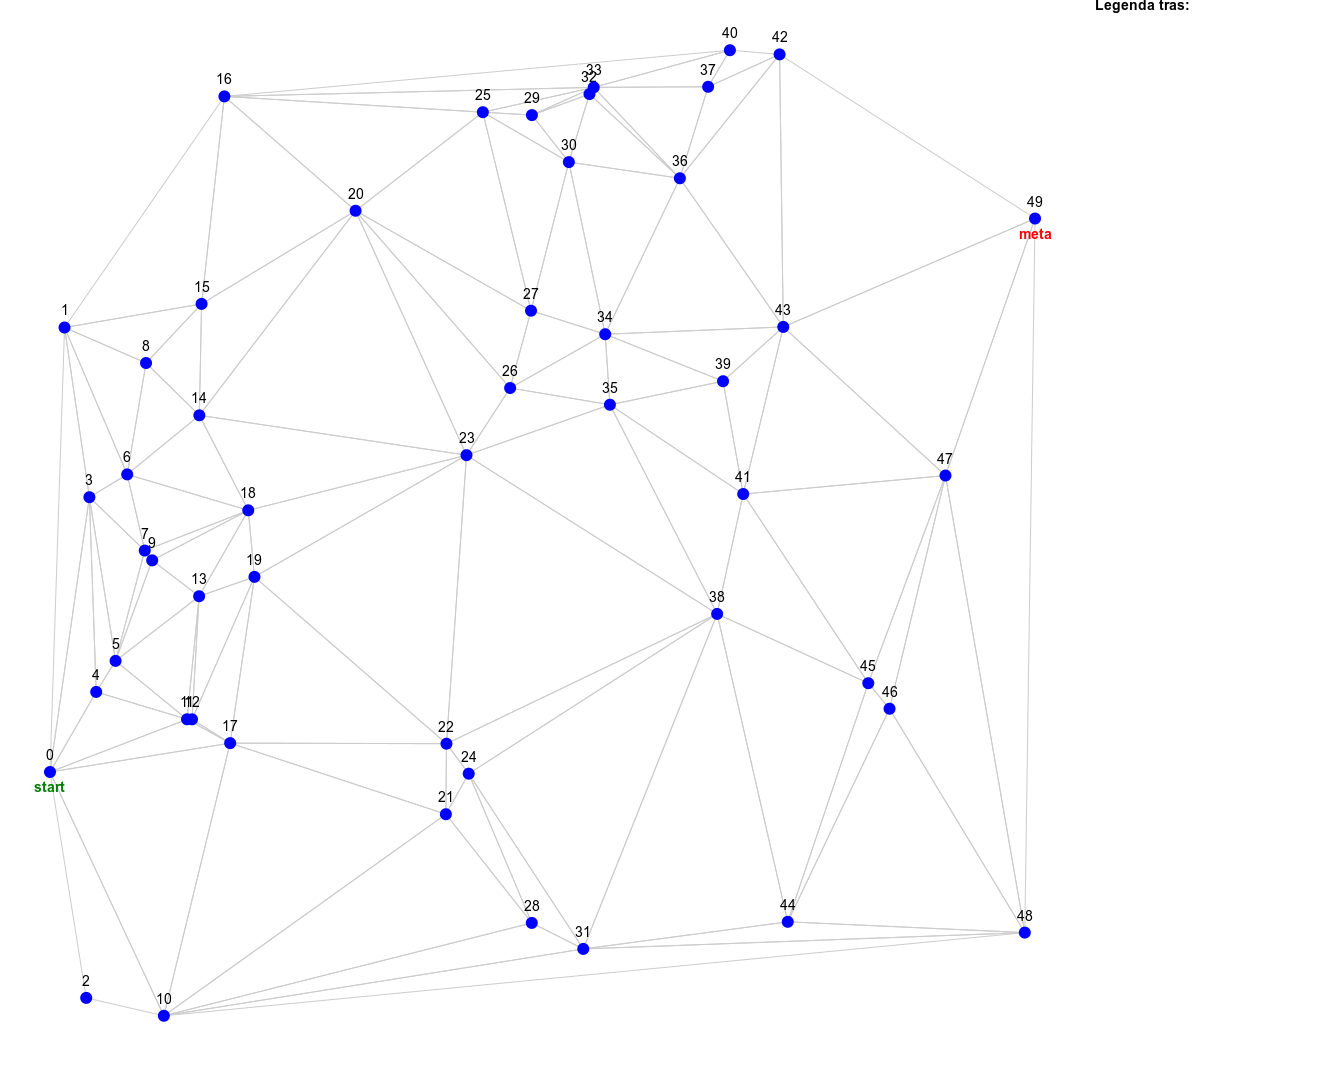
\includegraphics[width=1\linewidth]{375D41B5-CECC-49F4-95EB-B779CC90831A.png}
    \caption{Wizualizacja rozwiązania bez oznaczenia tras}
    \label{fig:enter-label}
\end{figure}

\begin{figure}[H]
    \centering
    \begin{minipage}[b]{0.48\linewidth}
        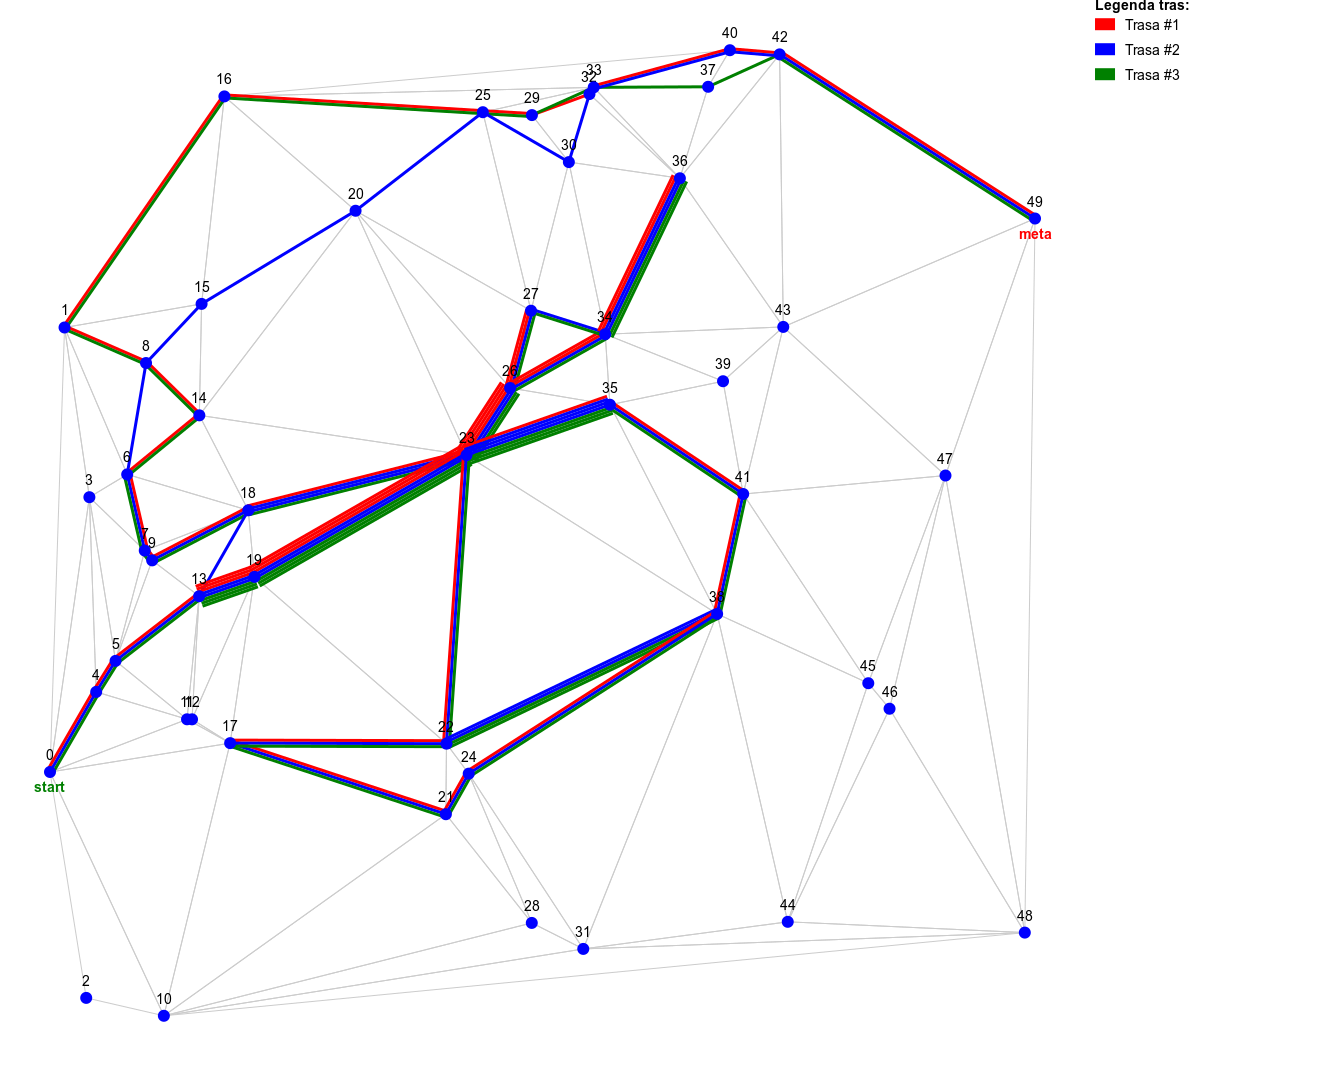
\includegraphics[width=\linewidth]{423C496B-894F-48DF-AD3A-845B3B00989B.png}
        \caption*{(a) Wizualizacja pierwszej trasy}
    \end{minipage}
    \hfill
    \begin{minipage}[b]{0.48\linewidth}
        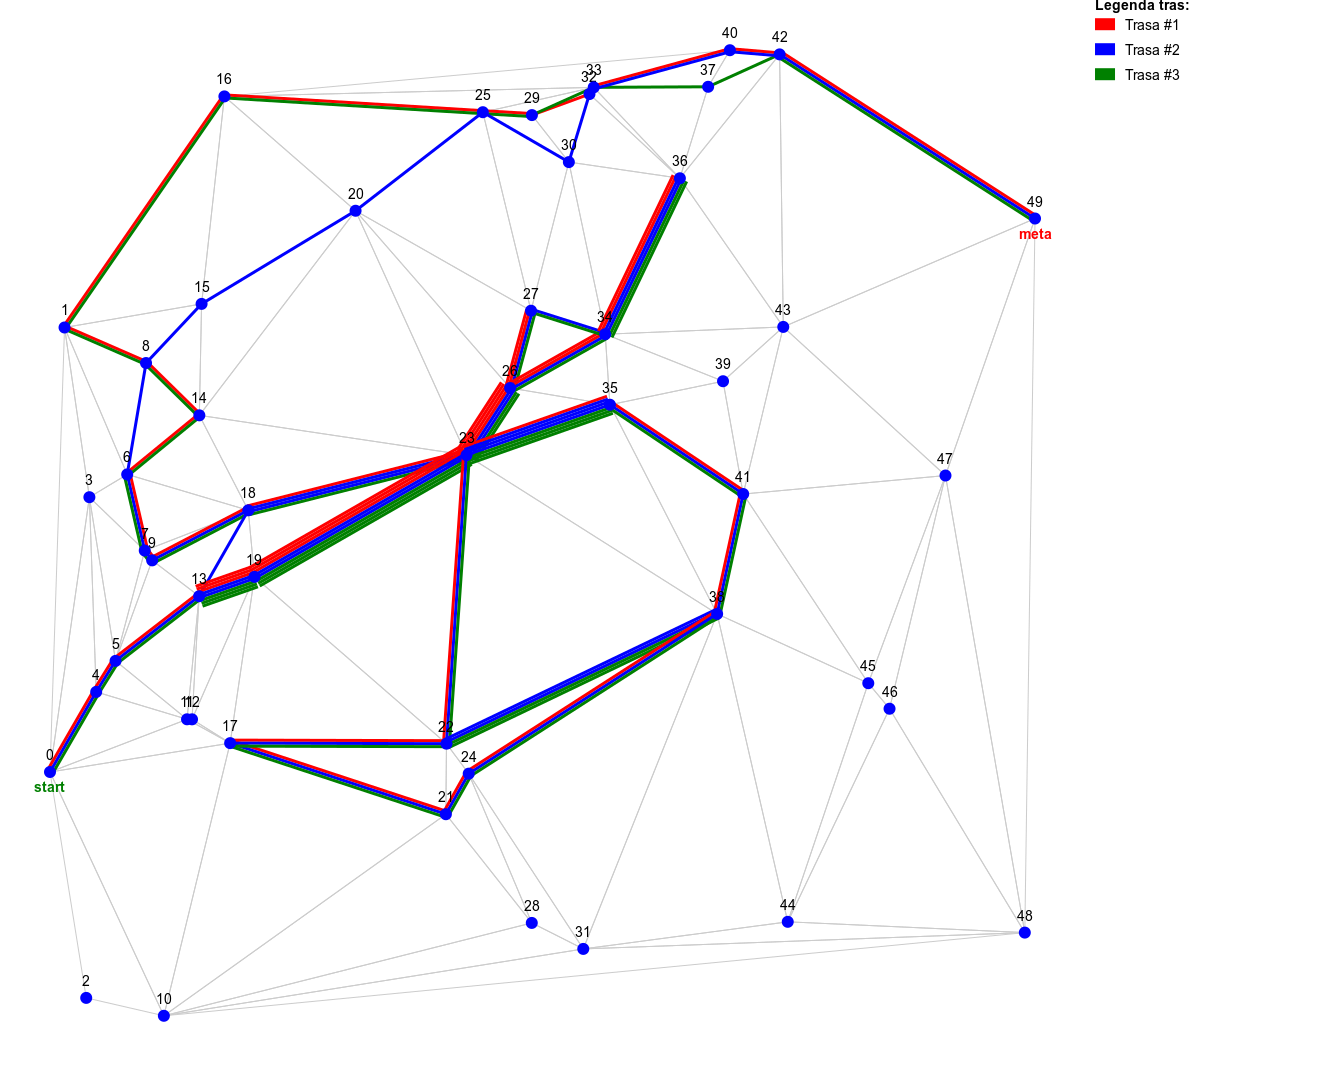
\includegraphics[width=\linewidth]{423C496B-894F-48DF-AD3A-845B3B00989B.png}
        \caption*{(b) Wizualizacja drugiej trasy}
    \end{minipage}

    \vspace{0.5em}
    \begin{minipage}[b]{0.48\linewidth}
        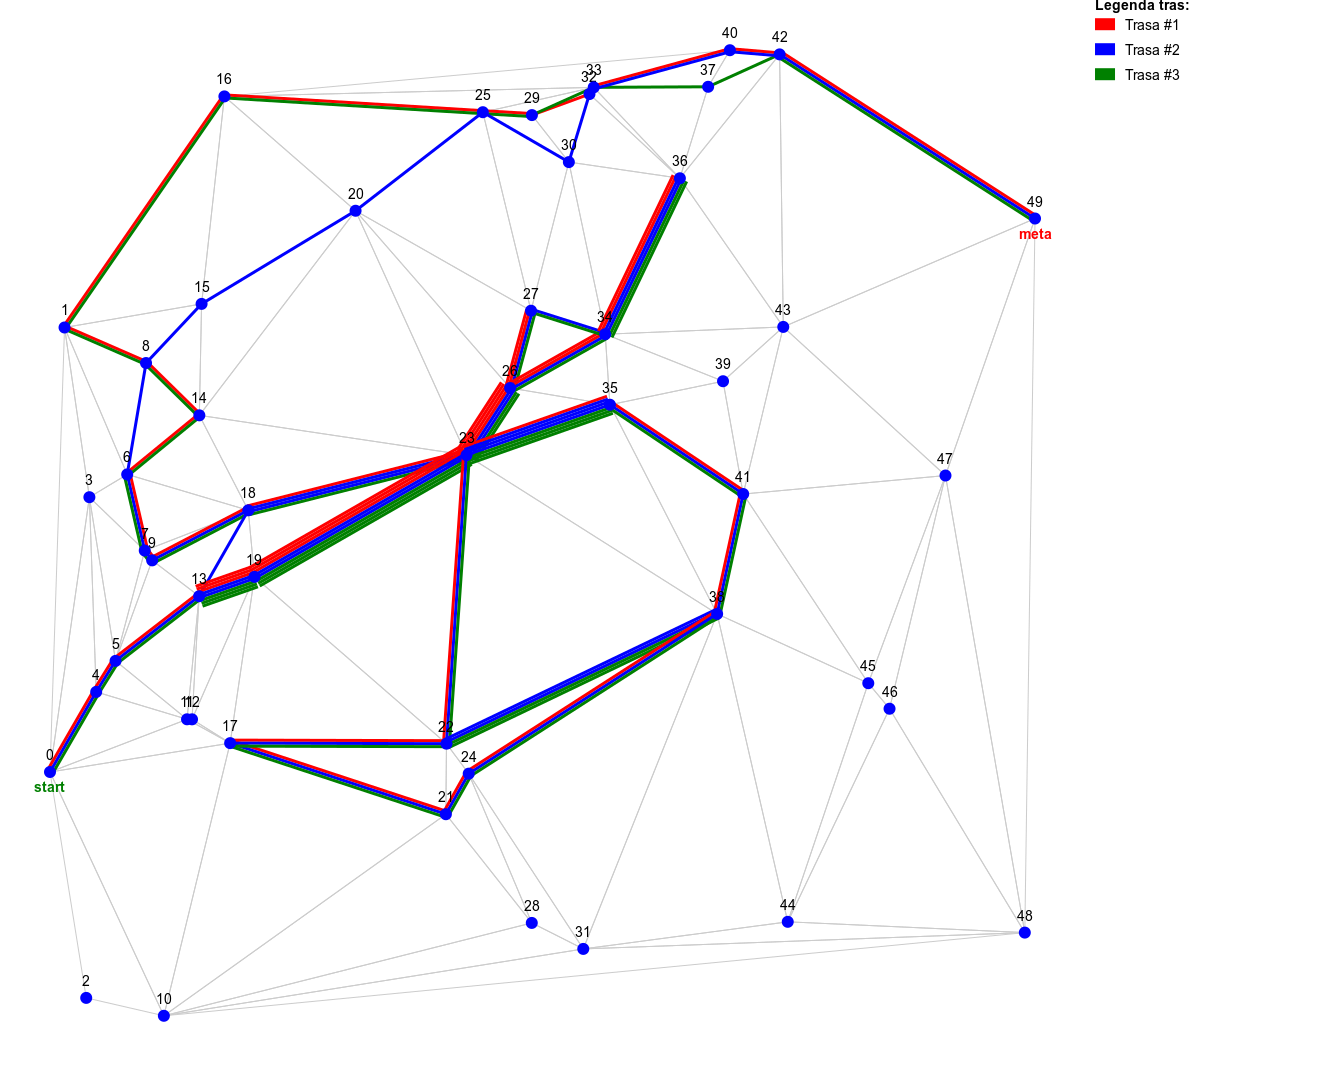
\includegraphics[width=\linewidth]{423C496B-894F-48DF-AD3A-845B3B00989B.png}
        \caption*{(c) Wizualizacja trzeciej trasy}
    \end{minipage}
    \hfill
    \begin{minipage}[b]{0.48\linewidth}
        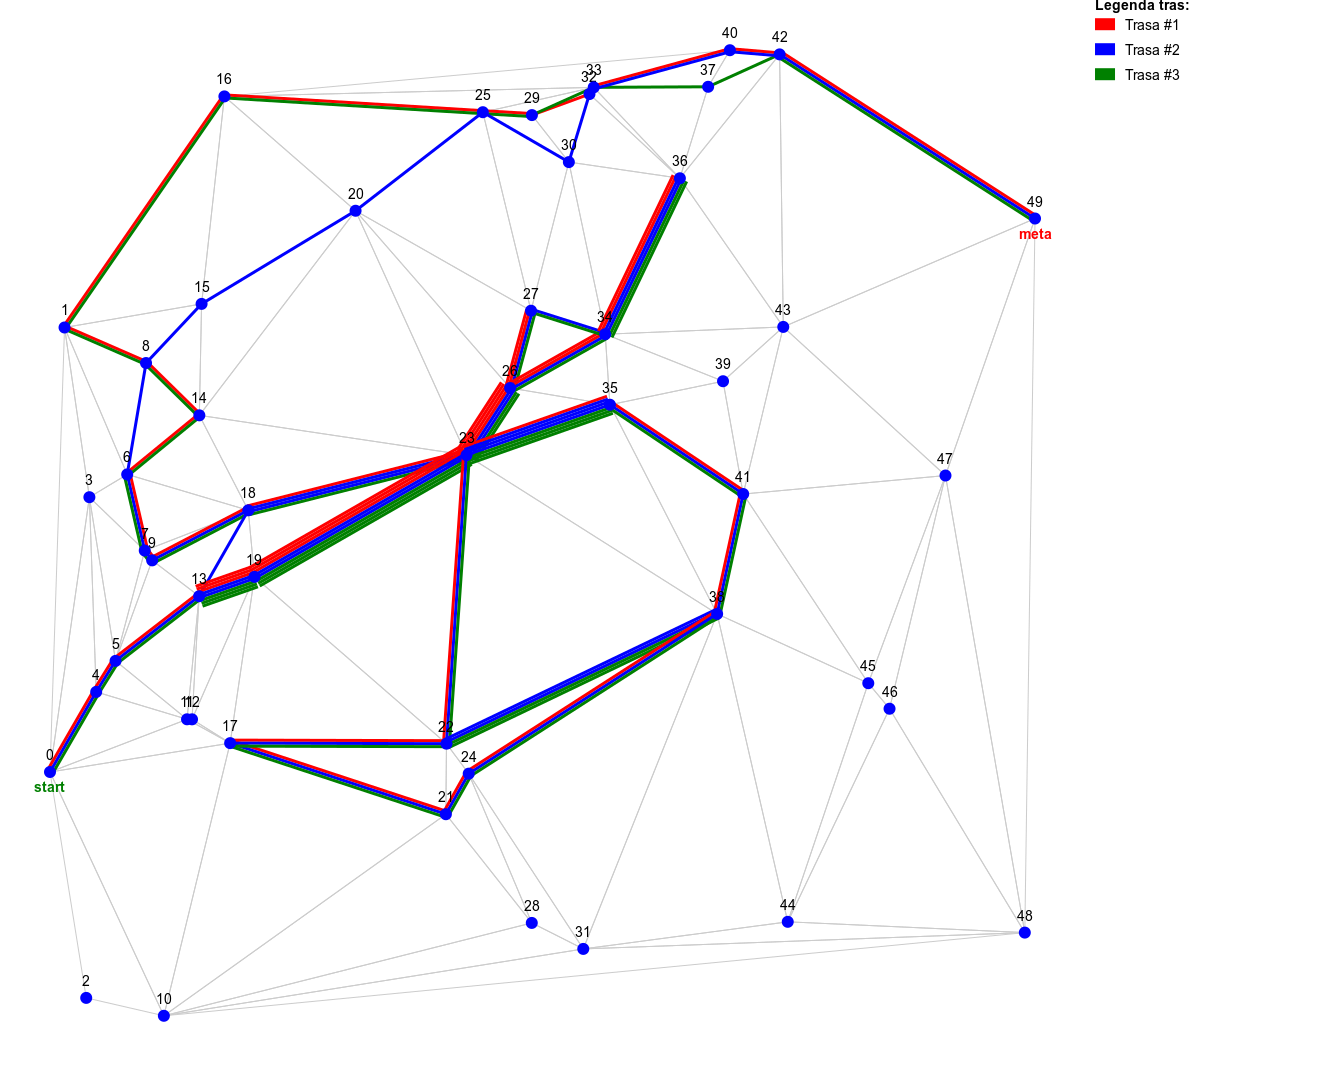
\includegraphics[width=\linewidth]{423C496B-894F-48DF-AD3A-845B3B00989B.png}
        \caption*{(d) Wizualizacja czwartej trasy}
    \end{minipage}

    \vspace{0.5em}
    \begin{minipage}[b]{0.48\linewidth}
        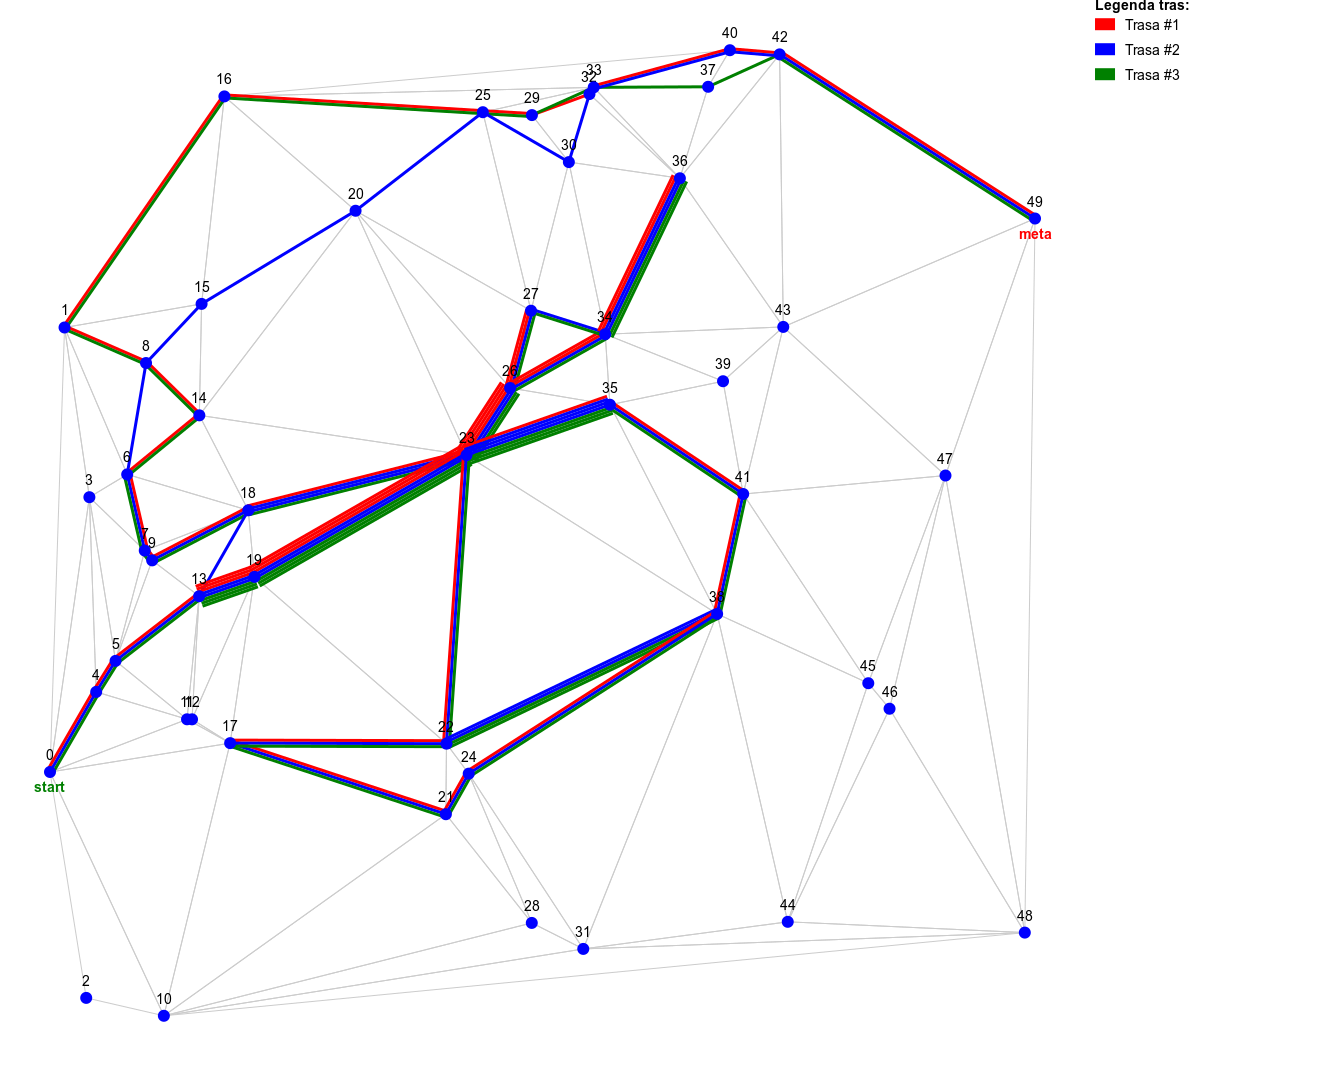
\includegraphics[width=\linewidth]{423C496B-894F-48DF-AD3A-845B3B00989B.png}
        \caption*{(e) Wizualizacja piątej trasy}
    \end{minipage}
    \hfill
    \begin{minipage}[b]{0.48\linewidth}
        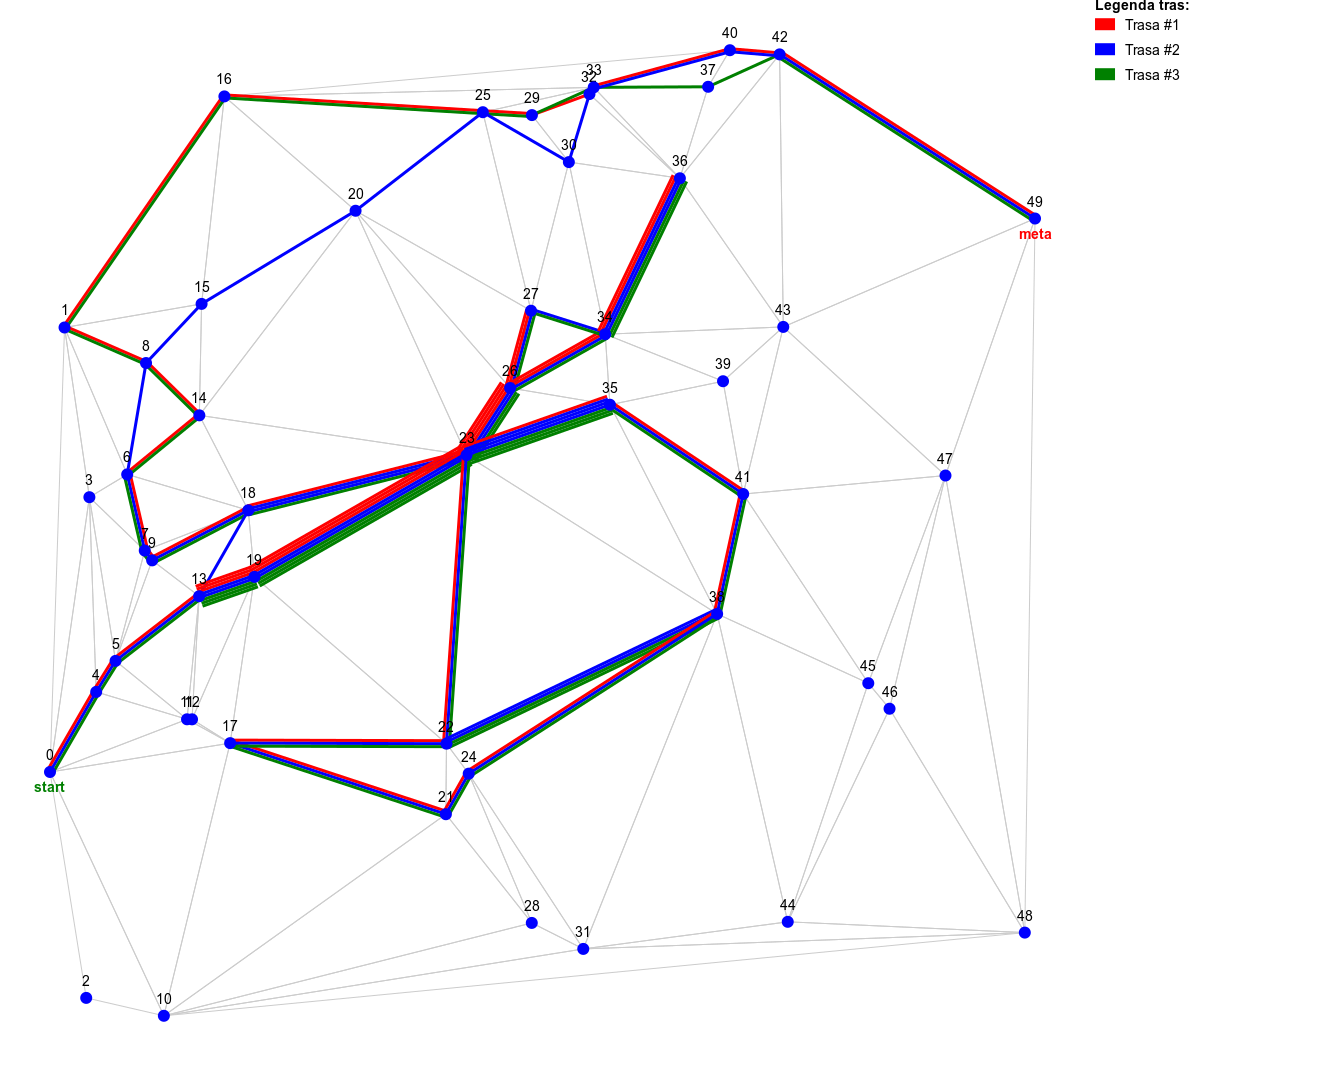
\includegraphics[width=\linewidth]{423C496B-894F-48DF-AD3A-845B3B00989B.png}
        \caption*{(f) Wizualizacja szóstej trasy}
    \end{minipage}
    
    \caption{Wizualizacje sześciu tras}
    \label{fig:all-routes}
\end{figure}

\subsection*{Uwagi końcowe}

Eksperyment potwierdził, że heurystyka Clarke’a-Wrighta potrafi wyznaczyć dobre jakościowo trasy, nawet w przypadku niestandardowego modelu z osobnym punktem startu i mety. Różnice w długości pomiędzy najlepszymi trasami wynikały z losowych permutacji listy oszczędności, co pokazuje elastyczność algorytmu.
\section{Podsumowanie}

Celem projektu było zaimplementowanie oraz przetestowanie heurystycznego rozwiązania problemu trasowania pojazdów (VRP) z oddzielnym punktem startu i końcowego powrotu. W tym celu wykorzystano zmodyfikowaną wersję algorytmu Clarke’a-Wrighta, który pozwala na skuteczne wyznaczanie tras w sposób szybki i skalowalny.

Na podstawie zebranych wyników oraz przeprowadzonych eksperymentów można sformułować następujące wnioski:

\begin{itemize}
    \item Algorytm oszczędnościowy okazał się skutecznym narzędziem do szybkiego generowania tras nawet w dużej instancji problemu (48 klientów).
    \item Dzięki implementacji wariantów z losową permutacją listy oszczędności, możliwe było znalezienie tras lepszych niż w podejściu deterministycznym.
    \item Struktura rozwiązania została zaprojektowana w sposób modularny, co umożliwia łatwą rozbudowę – zarówno pod kątem integracji z dokładnym solverem (np. CPLEX), jak i zastosowania innych heurystyk.
    \item Zastosowanie triangulacji i eksportu do formatu SVG umożliwiło przejrzystą wizualizację wyników, co znacznie ułatwia interpretację tras.
    \item Najlepsza trasa osiągnęła łączny koszt równy 221{,}302, przy pełnym pokryciu zbioru klientów – co jest wynikiem bardzo konkurencyjnym jak na rozwiązanie heurystyczne.
\end{itemize}

W kolejnych etapach projekt może zostać rozszerzony o:
\begin{itemize}
    \item pełne wsparcie dla wielu pojazdów,
    \item wprowadzenie ograniczeń czasowych (okien czasowych),
    \item uwzględnienie pojemności pojazdów,
    \item integrację z metodami optymalizacji dokładnej w celu dalszej poprawy wyników.
\end{itemize}

Uzyskane rezultaty potwierdzają praktyczną użyteczność heurystyki Clarke’a-Wrighta jako efektywnej metody inicjalizacyjnej lub samodzielnego rozwiązania dla problemów VRP średniej skali.
\end{document}